\section{ParaReal.jl}
\label{sec:impl:pr}

This section describes the general properties of the \julia{ParaReal.jl} package.
It has been designed with the following requirements in mind:
\begin{enumerate}
  \item\label{item:impl:goal:schedule}
    Schedule each stage on a separate process.

    This is a sensible default for the application at hand,
    which is memory bound for typical problem sizes.
    Yet, the scheduling strategy should be modifiable/extendable.
  \item\label{item:impl:goal:variablesize}
    Allow the data transferred be variable in size.

    This is necessary to transmit \ac{LRSIF} of varying rank and, therefore, storage size depending on $n$ (and $k$).
  \item\label{item:impl:goal:notransfer}
    Do not transfer the final solution data back to the calling/managing process.

    For fine resolutions, the storage requirements are immense.
    The overall solution might not fit in memory of a single compute node.
    Therefore, it has to be possible that each stage $n$ saves its local (fine) solution along $[t_{n-1},t_n]$ directly to disk,
    without sending it to the calling process first.
\end{enumerate}
On top of that:
\begin{enumerate}[resume]
  \item\label{item:impl:goal:modularity}
    The parareal implementation has to be modular,
    \ie easy to use/adapt for other problems than \ac{LRSIF} formulations of \ac{DRE}.
\end{enumerate}

Requirement \ref{item:impl:goal:schedule} is achieved by the abstract type \julia{Schedule},
whose sole subtype (for now) is \julia{ProcessesSchedule}.
It takes a list of $N$ worker/process ids, each of which will execute one stage.
Future strategies may be implemented by defining new subtype of \julia{Schedule}, \eg
\julia{ThreadsSchedule} using threads on a single process,
\julia{HybridSchedule} which uses both threads and processes, and
\julia{DaggerSchedule} which uses the abstractions provided by \julia{Dagger.jl}.\footnote{\url{https://github.com/JuliaParallel/Dagger.jl}}

Requirement \ref{item:impl:goal:variablesize} is trivial to fulfill using Julia's \julia{RemoteChannel} data type.
Requirement \ref{item:impl:goal:modularity} imposes a non-specific naming scheme for
user interface functions and the name of the unknown,
as to not clash with the standard nomenclatures of other disciplines.\footnote{%
  For example,
  many parareal papers use $U$ to name the unknown,
  many matrix \ac{ODE} papers use $X$,
  and the widely-used \julia{DifferentialEquations.jl} package~\cite{DifferentialEquations} uses $u$.
}
The next section will describe the user interface of the \julia{ParaReal.jl} package,
and how to cope with problem~\ref{item:impl:goal:notransfer}.

\subsection{User Interface}

In applications one is usually interested in a high temporal resolution,
while the parareal method is only used to obtain \enquote{fast} convergence.
Therefore, the \julia{ParaReal.jl} package distinguishes between a local solution along $[t_{n-1}, t_n]$ and the final value of which,
\begin{align*}
  F(U_{n-1}^k) &= \julia{value(fsolve(prob))} \\
  G(U_{n-1}^k) &= \julia{value(csolve(prob))}
\end{align*}
where \julia{prob} is an instance of the global \ac{IVP}~\eqref{eq:IVP}
restricted to the local time slice~$[t_{n-1}, t_n]$ and initial value~$U_{n-1}^k$.
The actual solver functions \julia{csolve} (\enquote{coarse}) and \julia{fsolve} (\enquote{fine})
are provided as arguments to \julia{ParaReal.Algorithm()}.
In order to support custom \ac{IVP} types,
a user has to defined methods for \julia{initial\_value()} to extract the global initial value $U_0$,
and \julia{remake\_prob()} to adjust the global problem for the local time slice and initial value.
For more details, refer to the documentation of the respective functions available from within Julia.

In order to support new solution types,
a custom implementation of the parareal update formula~\eqref{eq:pr:method} may be needed.
This can be specified as an optional third argument to \julia{ParaReal.Algorithm}.
The default is \julia{ParaReal.default\_update!()},
whose implementation is given in~\autoref{lst:impl:default_update!}.
Adding methods to \julia{default\_update!()} is not recommended.
Any custom implementation of the parareal update formula must follow the interface of \julia{default\_update!()}.

\def\sk{\textsuperscript{k}}
\def\skmi{\textsuperscript{k-1}}
\lstinputlisting[%
  float=t,
  label={lst:impl:default_update!},
  caption={Default implementations of the parareal update formula},
  escapechar=\%,
  breaklines=true,
]{code/default_update.jl}
% The form a+b+(-c) is for historical reasons. The LDLt data structure used to eagerly concatenate the
% matrices instead of collecting them lazily, as it does now. Back then, using a ternary plus meant
% fewer allocations (then: 2 allocs for L and 2 allocs for D, now: 0 allocs for L and 1 alloc for D)
% before compression.

The remainder of this section is devoted to a complete example of a user-defined problem type ($N=3$, $K=2$).
The problem type will be a mere placeholder that forwards its initial value,
while the solver functions will count the applications of $F$ and $G$ a particular solution is composed of.
Start by launching some worker processes and loading the necessary packages:
\lstinputlisting[%
  caption={User-defined problem type for \julia{ParaReal.jl}},
  label={lst:impl:parareal_counting},
  lastline=4,
]{code/parareal_counting.jl}
Next, define the problem type and ensure that definition is available on all processes.
The only requirement to the problem type is to have a \julia{tspan} field.\footnote{%
  Alternatively, it must support \julia{getproperty(prob, :tspan)}.
}
In the context of \ac{ODE}, this should not clash with any other notation.
\addtocounter{lstnumber}{1} %FIXME
\lstinputlisting[nolol, firstnumber=last, linerange=problem-end]{code/parareal_counting.jl}
The solution type will hold counters of the applications of $F$ and $G$:
\lstinputlisting[nolol, firstnumber=last, linerange=solution-end]{code/parareal_counting.jl}
Define the solver functions and problem instance and execute the parareal pipeline.
The solver functions are defined as closures,
such that they can be serialized and transferred to the worker processes.
Note that this code is only executed on the managing process:
\lstinputlisting[nolol, firstnumber=last, linerange=solve-end]{code/parareal_counting.jl}
Lastly, extracting the final values $U_1^1$, $U_2^2$, and $U_3^2$ via
\lstinputlisting[nolol, firstnumber=last, linerange=result-end]{code/parareal_counting.jl}
yields:
\begin{align*}
  &\julia{Counters(1,0)}, \text{ since} &
  U_1^1 &= F(U_0) \\
  &\julia{Counters(2,0)}, \text{ since} &
  U_2^2 &= F(F(U_0)) \\
  &\julia{Counters(3+2+2,2+4+4)}, \text{ since} &
  U_3^2 &= G(F(F(U_0))) + F(U_2^1) - G(U_2^1) \\
  && U_2^1 &= G(F(U_0)) + F(G(U_0)) - G(G(U_0))
\end{align*}

The full trajectory of the fine solver may be extracted using \julia{ParaReal.solution()}.
However, solution and value are identical in the example above,
\cf line~\ref{line:impl:parareal_counting:value}.
\autoref{lst:impl:store} shows the recommended pattern of
storing the fine solutions directly from the worker processes
via \julia{ParaReal.fetch\_from\_owner()}.

\lstinputlisting[%
  float=tpb, % TODO: ensure this doesn't disrupt the inline code snippets
  caption={%
    [Store fine parareal solutions directly from the worker processes]
    Store fine parareal solutions directly from the worker processes.
    This works well as a blueprint for \julia{DrWatson.\_wsave(dir, sol)} \cite{DrWatson}.
  },
  label={lst:impl:store},
]{code/parareal_store.jl}

\subsection{JIT Compilation and Warm-Up}
\label{sec:impl:pr:warmup}

Julia is a \ac{JIT} compiled language~\cite{Julia},
which means that code is compiled just before it is first executed,
unless it has already been compiled.
Therefore, unless the code has been compiled \ac{AOT},
only the second execution of code is fast.
This effect is called \emph{warm-up}.
As mentioned in~\autoref{sec:pr}, computing the coarse solutions
$G(U_n^*)$ is essentially a sequential operation over all $n$.
The computations of $F(U^*_n)$ can only be parallelized after such a global coarse solve.
Therefore, it is critical that the individual coarse solutions are available as fast as possible.

In order to describe the runtime of the present parareal implementation,
let $t_F$, $t_G$ denote the runtime of $F$ and $G$, respectively.
Let $N$ be the number of stages $1 \leq n \leq N$,
and $K$ be the number of refinements $0 \leq k \leq K$.
Let $\trampup$ be the overhead imposed on each computing the first coarse solution $G(U_n^0)$,
and $\twarmup$ be a general global overhead.
Further, we make the following assumptions:
\begin{enumerate}
  \item
    \label{item:impl:assumption:tF}
    $t_F$ and $t_G$ are constant, \ie do not depend on $n, k$.
  \item
    \label{item:impl:assumption:tU}
    The time to compute the actual value $U_n^k$ is negligible,
    \cf~\autoref{lst:impl:default_update!}.
  \item
    The overhead to check for convergence is negligible.
  \item
    Communication time is negligible.
  \item
    All stages $n$ compute $K$ refinements, \ie $k_n = K \enspace\forall n$.
\end{enumerate}
The runtime may then be estimated using
\begin{equation}
\label{eq:impl:tpar}
  \hattpar
  = \twarmup
  + \underbrace{
    \strut
    N \cdot (\trampup + t_G)
  }_{\substack{
    \text{stages $1\leq n\leq N$}\\
    \text{refinement $k=0$}
  }}
  + \underbrace{
    \strut
%TODO: Maybe k_N or (K-1) are more descriptive ...
    K \cdot (t_F + t_G)
  }_{\substack{
    \vphantom{\text{stage}}
    n = N \\
    1 \leq k \leq K
  }}
  + t_F
\end{equation}
where the final $t_F$ is to compute the best fine solution available.
These assumptions are compatible to the generic timeline \autoref{fig:timeline:generic}.
As will be described later,
\begin{equation}
  \twarmup + \trampup
  = t_{\JIT(G)} + t_\text{other}
\end{equation}
\ie the goal is to offset/reduce the ramp-up delay $\trampup$
at the cost of a one-time overhead $\twarmup$.
$t_{\JIT(G)}$ denotes the compile time of $G$.

\begin{figure}[p]
  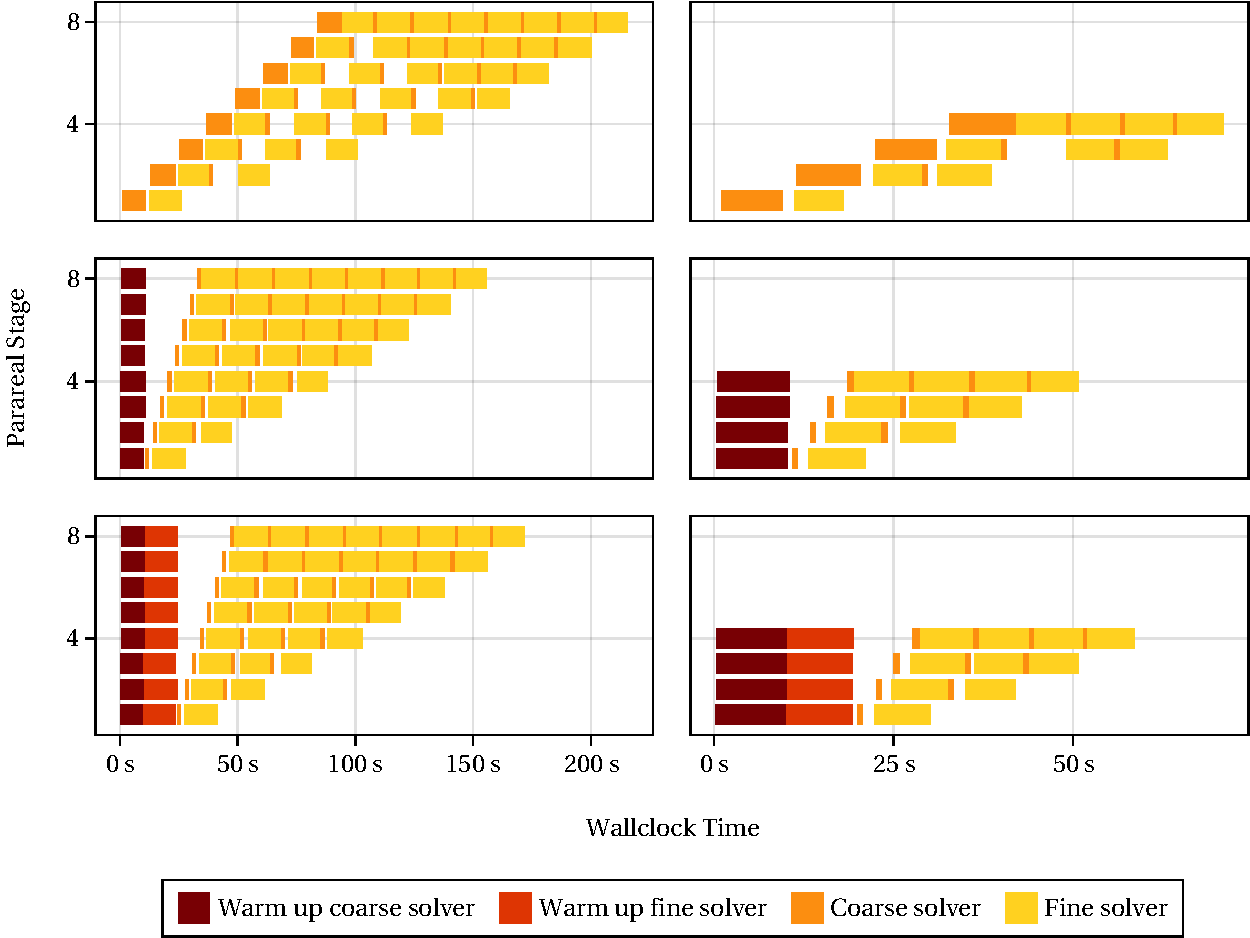
\includegraphics[width=\textwidth]{figures/fig_impl_warmup2.pdf}
  \caption[Timeline diagrams comparing the effect of JIT compiler warm-up]{%
    Timeline diagrams comparing the effect of \acs{JIT} compiler warm-up.
    Left: $N=8$ processes running on two compute nodes (4 threads/process),
    right: $N=4$ processes running on a laptop.
    Top: no warm-up,
    middle: warming up coarse solver $G$ (\julia{csolve}),
    bottom: warming up coarse and fine solver $F$ (\julia{fsolve}).
  }
  \label{fig:impl:warmup}
\end{figure}

\begin{table}[p]
  \centering
  \begin{tabular}{%
    lcc
    S[table-format=2.2]
    S[table-format=2.2]
    S[table-format=1.2]
    S[table-format=2.2]
    S[table-format=3.2]
    S[table-format=3.2]
    S[round-precision=3, round-minimum=0.001, table-format=<1.3, scientific-notation=fixed, fixed-exponent=0] % err
  }
    \toprule
    {warm-up} &
    {$N$} &
    {$K$} &
    {$\twarmup$} &
    {$\trampup$} &
    {$t_G$} &
    {$t_F$} &
    {$\tpar$} &
    {$\hattpar$} &
    {$\abs*{\frac{\hattpar-\tpar}{\tpar}}$} \\
    \midrule
    none & 8 & 7 & 0.0 & 10.448182003838676 & 1.3971984386444092 & 13.686557531356812 & 215.85136604309082 & 214.03589286123002 & -0.008410756045427896 \\
$G$ & 8 & 7 & 10.995897054672241 & 1.7753152676991055 & 1.3795734643936157 & 14.053897976875305 & 155.979896068573 & 158.32320497717177 & 0.015023147005871765 \\
$G$ and $F$ & 8 & 7 & 24.658120155334473 & 1.805815781865801 & 1.3864995241165161 & 13.99841558933258 & 171.88022804260254 & 171.88946398666928 & 5.373476735471789e-5 \\

    \addlinespace
    none & 4 & 3 & 0.0 & 9.887630144755045 & 0.6875278949737549 & 6.76188850402832 & 70.99208498001099 & 71.41076985994974 & 0.005897627602522728 \\
$G$ & 4 & 3 & 10.560525894165039 & 1.8285939693450928 & 0.7363770008087158 & 7.572427988052368 & 50.88027000427246 & 53.319252729415894 & 0.04793572685323071 \\
$G$ and $F$ & 4 & 3 & 19.362040996551514 & 1.843818744023641 & 0.6923139095306396 & 6.888918876647949 & 58.6095449924469 & 59.139188845952354 & 0.009036819063749955 \\

    \bottomrule
  \end{tabular}
  \caption[Timeline measurements comparing the effect of JIT compiler warm-up]{%
    Measurements corresponding to \autoref*{fig:impl:warmup}
    based on~\eqref{eq:impl:tpar}.
    The actual runtime is denoted by $\tpar$.
    $t_F$ and $t_G$ are estimated as the median,
    $\twarmup$ as the maximum of their respective runtimes.
    $\trampup$ is taken as the mean delay between adjacent $G(U_n^0)$ minus $t_G$.
    All timings are in seconds.
  }
  \label{tab:impl:warmup}
\end{table}

\paragraph{Sequential \ac{JIT} compilation}

Without any precautions,
\begin{equation*}
  \twarmup = 0,
\end{equation*}
\ac{JIT} compilation of $G$ happens sequentially,
as computing $G(U_n^k)$ is essentially sequential over $n$.
This effect is especially severe if the executors of different parareal iterations $(n,k)$ do not share the results of code compilation.
These executors may be processes, threads~(pthreads), or tasks~(green threads).
For the present implementation,
there is a one-to-one mapping between processes and stages $n$,
which means the compilation happens exactly once per stage $n$ and is reused between refinements $k$.\footnote{%
  As of the writing of this thesis, Julia does not reuse code compiled between processes.
}
This is visible in the first row of \autoref{fig:impl:warmup}
by the first occurrences of $G$ for each stage $n$,
which marks the computation of $G(U_n^0)$,
whose execution time includes compilation time.
Therefore, the first occurrences of $G$ take substantially longer than the subsequent ones.
The computation of the parareal update has a negligible duration,
and is therefore not shown in the timeline plot,
\cf assumption~\ref{item:impl:assumption:tU}.

\paragraph{Parallel \acs{AOT} compilation}

Since \julia{ParaReal.jl} is independent of $F$ and $G$ as well as the actual data type of the underlying \ac{IVP},
full \ac{AOT} compilation is difficult, and has to be done by users of the package.
A more naive approach is to manually warm up critical parts of the code by executing them before they are actually needed.
In the context of \julia{ParaReal.jl},
doing so allows to perform the compilation in parallel,
which significantly decreases the time to compute all coarse solutions $G(U_n^*)$.
This is visible in the middle and bottom rows of \autoref{fig:impl:warmup},
where
\begin{align*}
  \twarmup &= t_{\JIT(G)} + t_G
  \enspace
  \text{and} \\
  \twarmup &= t_{\JIT(G)} + t_G + t_{\JIT(F)} + t_F,
\end{align*}
respectively.
Warming up both $F$ and $G$ has (as expected) a negligible effect on~$\trampup$,
while adding a major overhead to~$\hattpar$ as generally $t_F \gg t_G$.

\paragraph{Precompilation}

Besides reducing the delay of executing $F$ and $G$,
it is also important to reduce the delay of any code from \julia{ParaReal.jl} that doesn't depend on them.
The package is merely responsible for orchestrating the execution of the parareal iterations $(n,k)$.
\todo{%
How to cite these webpages properly?
Should I do anything about the speculation in the paragraph, or the exposure of which in the footnote?
}
Therefore, the delay of the first execution of \julia{ParaReal.jl} code is dominated by type inference.\footnote{%
  At least it likely is. Taking measurements is highly non-trivial and out of the scope of this thesis.
  For more details see: \url{https://julialang.org/blog/2020/08/invalidations/}
}
The time spent on type inference can be minimized by precompilation,
which happens when the package is first loaded,
and whose results are cached and reused when the package is loaded again.
Exploiting this is highly non-trivial and out of the scope of this thesis.\footnote{\url{https://julialang.org/blog/2021/01/precompile_tutorial/}}

\paragraph{Numerical Results}

Refer to \autoref{tab:impl:warmup} for the measurements corresponding to \autoref{fig:impl:warmup}.
They are based on dense first-order Rosenbrock methods $G$ and $F$ applied to the Rail benchmark~\cite{morwiki_steel},
taking 1 step ($\tau=\SI{45}{\second}/N$) and 10 steps ($\tau=\SI{45}{\second}/10N$), respectively.
The relative errors in the final column show that the assumptions on \autopageref{item:impl:assumption:tU} are reasonable in this context.
Note that $K=N-1$, which is due to \autoref{thm:pr:conv}.

In the case of no warm-up, $\twarmup=0$, the overall compilation overhead caused by~$G$ scales linearly in~$N$.
If $G$ is instead being warmed up,
that overhead is constant and depends only on the underlying problem and solver.
$\trampup$ is significantly reduced in this case.
There is no point in warming-up $F$ as well.
However, the remaining $t_\text{other}$ includes compilation time for communications,
\eg to serialize the data types representing $U_n^k$,
and to establish a connection between adjacent pipeline stages.\footnote{%
  By default, connections between processes are established when they are first used.
  Here, only the connections between the calling process and the worker processes,
  each executing a pipeline stage,
  have been created.
}
This still leaves a linear overhead in the number of stages $N$
and potential for further improvements,
as ideally $\trampup=0$.
For the remainder of the thesis, $G$ will always be warmed up.

\subsection{Lack of Asynchronous Data Transfer}
\label{sec:impl:pr:sync}

A common strategy to improve CPU utilization is to perform data transfers between processes asynchronously.
Julia offers the \julia{RemoteChannel} data structure for this purpose.
As of the writing of this thesis,
the \julia{RemoteChannel} is not thread-safe.\footnote{\url{https://github.com/JuliaLang/julia/issues/37706}}
More specifically, it must be used from thread~1 of each process.
This means that in order to asynchronously send the interface~values~$U_n^{k+1}$ from stage $n$ to the next,
one would have to move the calls to~$F$ and~$G$ off of thread~1.
The reason is that many implementations of $F$ and $G$ don't have an implicit (cooperative) yield point to Julia's runtime,
such that no task can run asynchronously on thread~1 next to the task executing~$F$ and~$G$.
This is particularly true for code that doesn't require~\ac{IO},
\eg for many methods from Julia's \julia{LinearAlgebra} standard library,
which internally call \code{LAPACK}.

\todo{Mention that Julia runs single-threaded as to not oversaturate machine? BLAS/LAPACK launch their own threads.}
The solution described in the previous paragraph is not yet implemented,
\ie all data transfers are synchronous.
This causes gaps visible in \autoref{fig:impl:warmup} after $G$ and before $F$,
where the processor is essentially idle.
In general, a~gap ends shortly before $G$ starts on the next stage.\footnote{%
  There is one exception to this for $N=4$ and no warm-up.
  The last yellow box on stage $n=2$ in the top-right plot, $F(U_1^1)$,
  starts \enquote{too early} because $G(U_1^1)$ happens to finish before $G(U_2^0)$,
  and the Julia runtime has been able to schedule the receiving code one gap earlier.
}

Another effect is that the iterations $(n,k)$ for which $n+k \geq N$ show noticeably smaller gaps.
The reason is twofold.
The last stage $N$ doesn't need to send any data,
therefore has no \ac{JIT} warm-up delay for the first iteration $k=0$ and almost no gap in the diagram.
This causes the next refinement $k=1$ of the previous stage $N-1$ to have a noticeably smaller gap as well,
since its transmission code has already been compiled.
This effect propagates back-to-front through the still running pipeline stages.

The exact size of the gap between the computations of~$G(U_{n-1}^k)$ and~$F(U_{n-1}^k)$ of stage~$n$ is determined by
how much the stages are out-of-sync.
Assuming that
\begin{equation}
\label{eq:impl:assumption}
  t_F > t_G + t_{\JIT(G)}
\end{equation}
this includes for $n+k < N$
\begin{enumerate}
  \item\label{item:impl:comm:1}
    the overhead $t_\text{other}$,
    which includes \eg the compilation time of any transmission code,
    and
  \item\label{item:impl:comm:2}
    for $k\geq 1$ and no warm-up
    the overhead $t_{\JIT(G)}$ that,
    depending on the perspective,
    $G(U_n^{k-1})$ on the next stage finishes late,
    or $G(U_{n-1}^k)$ on the current stage finished early.\footnote{%
      Note how assumption~\eqref{eq:impl:assumption} is false for the hardware used in $N=4$,
      which causes the outlier described in the previous footnote.
    }
  %\item the time to compute the actual parareal value $U_n^k$.
\end{enumerate}
The last point causes the current stage to then \enquote{finish late} as well,
from the perspective of the previous stage.
For the first row of \autoref{fig:impl:warmup} effect~\ref{item:impl:comm:2} shadows~\ref{item:impl:comm:1},
while for the remaining rows effect~\ref{item:impl:comm:2} is essentially zero.

\subsection{Early Convergence}
\label{sec:impl:pr:conv}

Due to \autoref{thm:basics:dre-limit-are},
later parareal stages are expected to require fewer Newton refinements than earlier stages to reach convergence.
Therefore, each stage $n$ may defer the computation of a refinement $k$,
until the previous stage $n-1$ finished computing its refinement $k+1$.
That is, the number of refinements computed may differ by at most one from stage to stage,
\ie $k_{n+1} \geq k_n -1$ where $k_n$ denotes the last refinement computed by stage $n$.
These effects are best to be seen in \autoref{fig:impl:restart},
which corresponds to the reference solution of \autoref{fig:results:parareal:rail} to be described in \autoref{sec:results:parareal}.
This timeline also shows when the stages~$n$ are waiting for input,
which may be a new initial value~$U_{n-1}^k$ or the signal that the previous stage finished.
In that case, stage~$n$ may safely finish as well,
since~$k_{n-1}$ won't increase any further.

To summarize all effects described so far,
the revised schematic timeline plot is shown in \autoref{fig:timeline:revised},
\cf \autoref{fig:timeline:generic} for the expected schematic timeline.
With respect to \autoref{fig:impl:warmup},
the faces $k=K$ and therefore early convergence are not visible.
The face $n+K \geq N$ is most pronounced in the top left diagram.
For large $N$, $N \gg K$, that effect will be negligible for the overall runtime of the parareal algorithm.

\begin{figure}[tp]
  \centering
  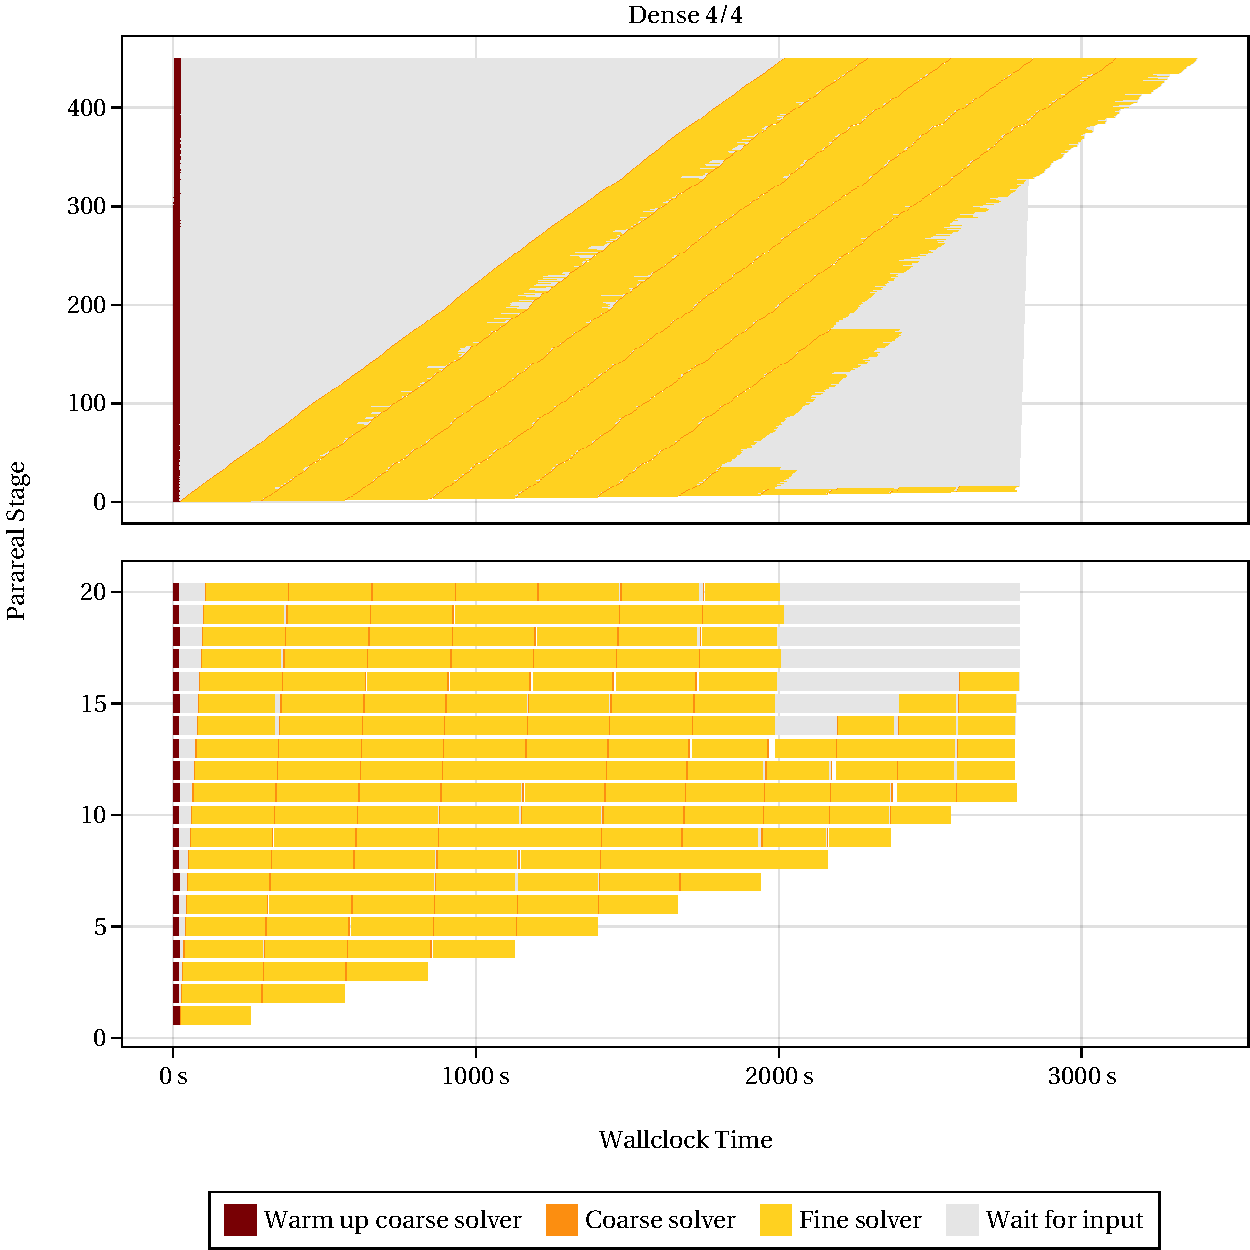
\includegraphics[width=\textwidth]{figures/fig_timeline_ref.pdf}
  \caption[Restarted parareal computation]{
    Restarted parareal computations to maintain $k_{n+1} \geq k_n - 1$.
    Top: full timeline of parareal algorithm applied to Rail benchmark~\cite{morwiki_steel}, $N=450$.
    Bottom: zoom to first stages $1 \leq n \leq 20$.
  }
  \label{fig:impl:restart}
\end{figure}

\begin{figure}[t]
  \centering
  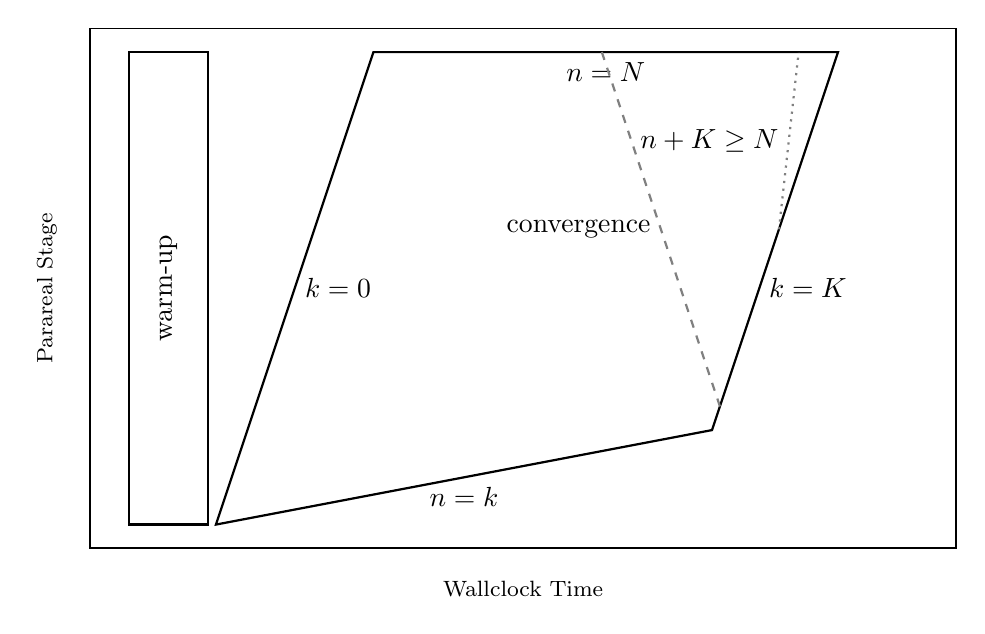
\begin{tikzpicture}
  \def\myscale{0.6}
  % axis and labels
  \node[below] at (5,-0.5*\myscale-0.3) {\footnotesize Wallclock Time};
  \node[rotate=90, above] at (-0.5-0.3,5*\myscale) {\footnotesize Parareal Stage};
\begin{scope}[yscale=\myscale]
  \draw[semithick] (-0.5,-0.5) rectangle (10.5,10.5);
  % timeline diagram
  \draw[thick] (0,0) rectangle node[rotate=90] {warm-up} (1,10);
  \draw[thick] (1.1,0)
    -- node[right] {$k=0$} (3.1,10)
    -- node[below] {$n=N$} (9,10)
    -- (7.4,2)
    -- node[below] {$n=k$} cycle;
  \node[right] at (8,5) {$k=K$};
  % lack of asynchronous data transfer
  \draw[thick,gray,dotted] (8.25,6.25)
    -- node[black,left] {$n+K \geq N$} (8.5,10);
  % early convergence due to "delta k = 1"
  \draw[thick,gray,dashed] (7.5,2.5)
    -- node[black,left] {convergence} (6,10);
\end{scope}
\end{tikzpicture}

  \caption[Revised schematic timeline diagram]{%
    Revised schematic timeline diagram of \julia{ParaReal.jl} implementation for $N$ stages and $K$ refinements.
    The dotted line is due to the lack of asynchronous data transfer for $n+k \geq N$,
    \cf~\autoref{sec:impl:pr:sync}.
    The dashed line indicates early convergence for $k_n < k_{n+1}$,
    \cf~\autoref{sec:impl:pr:conv}.
  }
  \label{fig:timeline:revised}
\end{figure}

\subsection{Parallel Scaling}

Common metrics to compare parallel codes with are \emph{speedup}~$\tseq/\tpar$
and \emph{parallel efficiency}~$\tseq/P\cdot\tpar$
where $\tseq$ denotes the runtime of the fastest sequential algorithm,
$\tpar$ the runtime of a parallel algorithm solving the same problem,
and $P\in\N$ denotes the number of processors the parallel code is executed on.
These timings, and therefore the metrics as well, depend on the size of the problem.
Usually, $\tseq$ is not available and therefore estimated as the sequential runtime of the parallel algorithm.

In the context of the parareal method,
the size of the problem refers to the number of steps of the fine solver or the resolution of the output trajectory.
Instead of estimating $\tseq$ as the sum of all $F$ and $G$ evaluated,
a more relevant comparison is the theoretical runtime of the fine solver $F$ over the whole time span.
Therefore, let $\hattseq$ be the total duration of the most recent fine solutions computed,
\begin{equation}
\label{eq:impl:tseq}
  \hattseq = \sum_{n=1}^N t_F(n, k_n)
\end{equation}
where $k_n$ is the latest refinement $k$ computed on stage $n$,
and $t_F(n,k)$ denotes the runtime of $F(U_{n-1}^k)$.
In \autoref{sec:impl:pr:warmup},
$t_F(n,k)$ had been assumed to be constant,
\cf~assumption~\ref{item:impl:assumption:tF} on \autopageref{item:impl:assumption:tF}.
However, as will be described in the next section,
for the \ac{LRSIF} methods this is not true.

As mentioned at the beginning of \autoref{sec:impl:pr},
there is a one-to-one mapping between stages $n$ and processes.
This means that the parallel efficiency has to be evaluated for $P=N$,
which yields very low parallel efficiencies.
Despite that, the speedups are quite good from a user's/engineer's perspective for larger $N$.
Refer to \autoref{tab:impl:pr:speedup} for the measurements corresponding to the numerical results
to be discussed in the next section.

% TODO: for defense
% post-mortem scheduling (\eg naive round-robin) to obtain a minimum $\hat P$ necessary to obtain the \emph{same} timeline.
% Use that to compute hypothetical parallel efficiencies.

As early stages $n \leq K$ only compute $k=n$ refinements,\footnote{%
  Technically, they only compute $k=n-1$ refinements and then directly take the fine solution $F(U_{n-1}^{n-1})$,
  which had already been evaluated for $U_n^{n-1}$,
  \cf \autoref{thm:pr:conv}.
}
their processes become idle even before late stages receive their first $U^0_n$,
\cf \eg left column of \autoref{fig:impl:warmup}.
These processes may easily be reused,
resulting in fewer processors being necessary, $P < N$,
to obtain the same timeline.
However, these processes must be warmed up only once,
since the warm-up calls to $G$ would not be executed in parallel.
Refer to \eg \cite{Nielsen2018} for a more advanced scheduling strategy to better utilize given hardware.

\subsection{Parallel Programming Pitfalls}

\begin{itemize}
  \item
    \julia{@sync} may block\footnote{\url{https://github.com/JuliaLang/julia/issues/32677}}
    There is an experimental eager version,\footnote{\url{https://github.com/JuliaLang/julia/pull/34198}} but it doesn't support cancellation.
    In general, as of the time of writing this thesis,
    there is no recommended way to handle cancellation using the standard library,
    especially (and frustratingly) in a distributed environment.
  \item
    By default, unhandled concurrent errors are transient.\footnote{%
      \url{https://github.com/JuliaLang/julia/issues/10405}}
    That means that if a background task fails, not only does the program keep running, it doesn't even print an error.\footnote{%
      \url{https://github.com/JuliaLang/julia/pull/27722}}
    It is not easy to let unhandled concurrent errors crash the whole program.
    More severly, in a distributed environment, a failed task on one machine may easily cause a different machine to deadlock,
    \cf the previous paragraph.
    It is the user's (or the library developer's) responsibility to make errors observable,\footnote{%
      \url{https://github.com/JuliaLang/julia/pull/39518}}
    and to make sure that whole computation is properly cancelled.
  \item
    \url{https://github.com/JuliaLang/julia/issues/38931},
    \url{https://github.com/JuliaLang/julia/pull/44671}
\end{itemize}

